%
% CMPT 454: Database Systems II - A Course Overview
% Section: External Sorting
%
% Author: Jeffrey Leung
%

\section{External Sorting}
	\label{sec:external-sorting}
\begin{easylist}

& Sorting is essential for:
	&& Outputting data in sorted order
	&& Removing duplicates
	&& Preparing data for B+ tree insertion

& B+ tree: If the data to be retrieved is clustered, then it is efficient to retrieve as sorted

& Evaluation strategy is chosen before query execution, for optimized performance

& \textbf{External sort:} Sorting algorithm which operates on primitive data pages but is not executed by the database
	&& \textbf{Run:} Sorted subfile used during a larger sort strategy
	&& \textbf{Input buffer:} Memory slot which holds data to be processed
	&& \textbf{Output buffer:} Memory slot which holds data to be written to the disk

\end{easylist}
\subsection{Merge Sort}
	\label{subsec:merge-sort}
\begin{easylist}

& Merge sort: External sorting algorithm
	&& Process:
		&&& On the first pass:
			&&&& Read pages (up to the number of buffers)
			&&&& Sort each page individually
			&&&& Write pages back to disk
			
		&&& On subsequent passes:
			&&&& Reserve a single buffer for output
			&&&& Merge two `runs' into a single run, in the output buffer
				&&&&& Given $B$ available buffers, $B-1$ runs can be merged in a single pass
			&&&& Write the output buffer back to disk
			&&&& Repeat
		&&& Diagram: See figure~\ref{img:merge-sort}

		\begin{figure}[!htb]
			\centering
			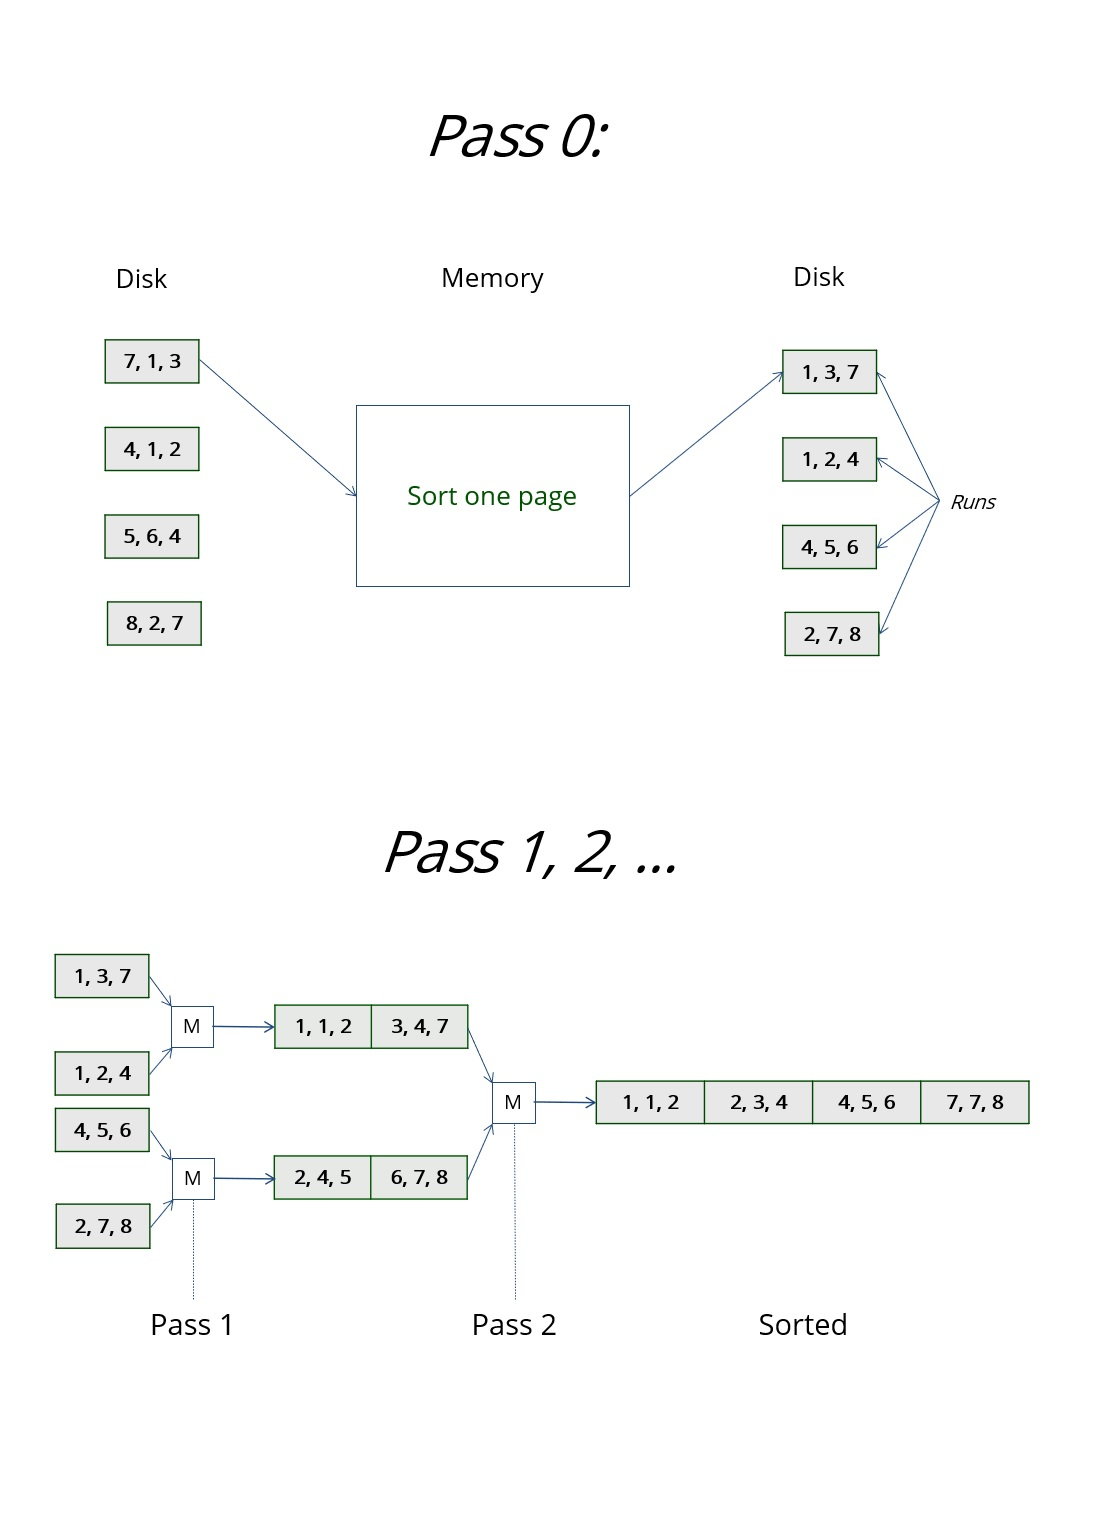
\includegraphics[width=.8\linewidth]{external-sorting/merge-sort}
			\caption{Diagram of the First and Subsequent Passes of a Merge Sort}
			\label{img:merge-sort}
		\end{figure}

& Page I/O (given $n$ data pages to sort):
	&& $n$ for the first pass
	&& $2n$ for each subsequent pass (as each processed value is read once and written once)
	
& Buffer management:
	&& Given $n$ available buffers:
		&&& One buffer is used as an sorted output buffer (written to disk whenever full and emptied)
		&&& $n-1$ buffers are used to track one run each, from which data is fed into the output buffer
	&& Merge as many buffers as possible during each pass, to minimize time

\clearpage
\end{easylist}
\subsection{Replacement Sort}
	\label{subsec:replacement-sort}
\begin{easylist}
	
& \textbf{Replacement sort:} External sorting algorithm where a sorted run is continuously built from a current working set of available data
	&& Consists of one input buffer, one `current set' of sortable data, and one output buffer
	&& Process:
		&&& Whenever the input buffer is empty, fill it with a new page from the disk
		&&& Whenever the current set has an empty slot, fill it with data from the input buffer
		&&& From the current set, take the value which meets the following conditions and add it to the output buffer:
			&&&& The minimum possible value in the set, and
			&&&& Equal or greater than the maximum value in the output buffer
		&&& Whenever the output buffer is full, write it to disk and empty it
		&&& Repeat until all data has been read from the disk once (completing one round)
		&&& Repeat rounds until the current set is empty at the end of the round

& Diagram: See figure~\ref{img:replacement-sort}

\begin{figure}[!htb]
	\centering
	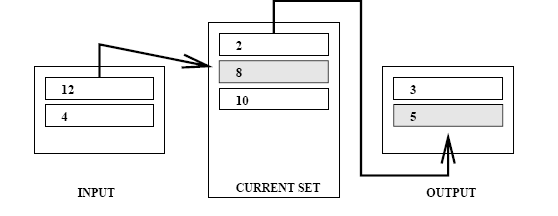
\includegraphics[width=.8\linewidth]{external-sorting/replacement-sort}
	\caption{Diagram of the Replacement Sort Data Structure}
	\label{img:replacement-sort}
\end{figure}

\end{easylist}
\clearpage